\documentclass[a4paper,11pt,fleqn]{article}

\usepackage[left=1cm,right=1cm,top=0.5cm,bottom=2cm]{geometry}

\usepackage{bfcours}
\usepackage{bfcours-fonts}
%\usepackage{bfcours-fonts-dys}

\def\rdifficulty{1}
\setrdexo{%left skip=1cm,
display exotitle,
exo header = tcolorbox,
%display tags,
skin = bouyachakka,
lower ={box=crep},
display score,
display level,
save lower,
score=\points,
level=\rdifficulty,
overlay={\node[inner sep=0pt,
anchor=west,rotate=90, yshift=0.3cm]%,xshift=-3em], yshift=0.45cm
at (frame.south west) {\thetags[0]} ;}
]%obligatoire
}
\setrdcrep{seyes, correction=true, correction color=monrose, correction font = \large\bfseries}

\newcommand{\tikzinclude}[1]{%
    \stepcounter{tikzfigcounter}%
    \csname tikzfig#1\endcsname
}
\newcommand{\tikzfigTnVi}{
\begin{tikzpicture}[line cap=round,line join=round,>=triangle 45,x=1.0cm,y=1.0cm,scale=0.6]
\begin{axis}[
x=1.0cm,y=1.0cm,
axis lines=middle,
ymajorgrids=true,
xmajorgrids=true,
xmin=-1.5,
xmax=3.5,
ymin=-3.2,
ymax=3.2,
xtick={-1.0,0.0,...,3.0},
ytick={-3.0,-2.0,...,3.0},]
\clip(-1.5,-3.2) rectangle (3.5,3.2);
\draw[line width=2.pt,color=blue,smooth,samples=100,domain=-1.5:3.5] plot(\x,{-0.6*((\x)-1.0)^(2.0)+2.0});
\begin{scriptsize}
\draw[color=blue] (-1,1) node {\large{$\mathcal{C}_f$}};
\end{scriptsize}
\end{axis}
\end{tikzpicture}
}

\newcommand{\tikzfigXWyE}{
\begin{tikzpicture}[line cap=round,line join=round,>=triangle 45,x=1.0cm,y=1.0cm,scale=0.6]
\begin{axis}[
x=1.0cm,y=1.0cm,
axis lines=middle,
ymajorgrids=true,
xmajorgrids=true,
xmin=-1.5,
xmax=3.5,
ymin=-3.2,
ymax=3.2,
xtick={-1.0,0.0,...,3.0},
ytick={-3.0,-2.0,...,3.0},]
\clip(-1.5,-3.2) rectangle (3.5,3.2);
\draw[line width=2.pt,color=blue,smooth,samples=100,domain=-1.5:3.5] plot(\x,{0.5*((\x)-2.0)^(2.0)-3.0});
\begin{scriptsize}
\draw[color=blue] (-1,2.5) node {\large{$\mathcal{C}_g$}};
\end{scriptsize}
\end{axis}
\end{tikzpicture}
}

\newcommand{\tikzfigbxUA}{
\begin{tikzpicture}[line cap=round,line join=round,>=triangle 45,x=1.0cm,y=1.0cm,scale=0.6]
\begin{axis}[
x=1.0cm,y=1.0cm,
axis lines=middle,
ymajorgrids=true,
xmajorgrids=true,
xmin=-1.5,
xmax=3.5,
ymin=-3.2,
ymax=3.2,
xtick={-1.0,0.0,...,3.0},
ytick={-3.0,-2.0,...,3.0},]
\clip(-1.5,-3.2) rectangle (3.5,3.2);
\draw[line width=2.pt,color=blue,smooth,samples=100,domain=-1.5:3.5] plot(\x,{0-0.3*((\x)-1.0)^(2.0)-1.0});
\begin{scriptsize}
\draw[color=blue] (2.5,-1) node {\large{$\mathcal{C}_h$}};
\end{scriptsize}
\end{axis}
\end{tikzpicture}
}

\newcommand{\tikzfigzaPA}{
\begin{tikzpicture}[line cap=round,line join=round,>=triangle 45,x=1.0cm,y=1.0cm,scale=0.6]
\begin{axis}[
x=1.0cm,y=1.0cm,
axis lines=middle,
ymajorgrids=true,
xmajorgrids=true,
xmin=-1.5,
xmax=3.5,
ymin=-3.2,
ymax=3.2,
xtick={-1.0,0.0,...,3.0},
ytick={-3.0,-2.0,...,3.0},]
\clip(-1.5,-3.2) rectangle (3.5,3.2);
\draw[line width=2.pt,color=blue,smooth,samples=100,domain=-1.5:3.5] plot(\x,{0-1*((\x)+0.0)^(2.0)+2.0});
\begin{scriptsize}
\draw[color=blue] (-1,2.5) node {\large{$\mathcal{C}_i$}};
\end{scriptsize}
\end{axis}
\end{tikzpicture}
}

\newcommand{\tikzfigmWht}{
\begin{tikzpicture}[line cap=round,line join=round,>=triangle 45,x=1.0cm,y=1.0cm,scale=0.8]
\clip(2.5,0.5) rectangle (9.5,5.5);
\fill[line width=2.pt,color=ffffff,fill=ffffff,fill opacity=1.0] (3.,5.) -- (9.,5.) -- (9.,1.) -- (3.,1.) -- cycle;
\fill[line width=0.pt,color=ffqqqq,fill=ffqqqq,fill opacity=1.0] (3.,5.) -- (3.,3.5) -- (4.5,3.5) -- (4.5,5.) -- cycle;
\fill[line width=0.pt,color=ffqqqq,fill=ffqqqq,fill opacity=1.0] (3.,1.) -- (3.,2.5) -- (4.5,2.5) -- (4.5,1.) -- cycle;
\fill[line width=0.pt,color=ffqqqq,fill=ffqqqq,fill opacity=1.0] (5.5,1.) -- (5.5,2.5) -- (9.,2.5) -- (9.,1.) -- cycle;
\fill[line width=0.pt,color=ffqqqq,fill=ffqqqq,fill opacity=1.0] (5.5,5.) -- (5.5,3.5) -- (9.,3.5) -- (9.,5.) -- cycle;
\draw [line width=2.pt] (3.,5.)-- (9.,5.);
\draw [line width=2.pt] (9.,5.)-- (9.,1.);
\draw [line width=2.pt] (9.,1.)-- (3.,1.);
\draw [line width=2.pt] (3.,1.)-- (3.,5.);
\end{tikzpicture}
}

\newcommand{\tikzfigFuya}{
\begin{tikzpicture}[line cap=round,line join=round,>=triangle 45,x=1.0cm,y=1.0cm,scale=1]
\clip(-0.1,-0.1) rectangle (4.1,4.1);
\fill[line width=1.pt,color=blue,fill=blue!30,fill opacity=1] (0,0) -- (3.,0.) -- (0.,1.) -- cycle;
\fill[line width=1.pt,color=red,fill=blue!30,fill opacity=1] (4,0) -- (4,3) -- (3,0) -- cycle;
\fill[line width=1.pt,color=blue,fill=blue!30,fill opacity=1] (4,4) -- (1,4) -- (4,3) -- cycle;
\fill[line width=1.pt,color=blue,fill=blue!30,fill opacity=1] (0,4) -- (0,1) -- (1,4) -- cycle;
\draw [line width=1.pt,color=blue] (0,0)-- (4,0);
\draw [line width=1.pt,color=blue] (4,0)-- (4,4);
\draw [line width=1.pt,color=blue] (4,4.)-- (0,4);
\draw [line width=1.pt,color=blue] (0,4)-- (0,0);
\draw [line width=1.pt,color=blue] (0,1)-- (3,0);
\draw [line width=1.pt,color=blue] (3,0)-- (4,3);
\draw [line width=1.pt,color=blue] (4,3)-- (1,4);
\draw [line width=1.pt,color=blue] (1,4)-- (0,1);
\end{tikzpicture}
}



\hypersetup{
    pdfauthor={R.Deschamps},
    pdfsubject={},
    pdfkeywords={},
    pdfproducer={LuaLaTeX},
    pdfcreator={Boum Factory}
}



\begin{document}

\setcounter{pagecounter}{0}
\setcounter{ExoMA}{0}


\def\rdifficulty{1}
\chapitre[
    $\mathbf{1^{\text{ère}}}$% : $\mathbf{6^{\text{ème}}}$,$\mathbf{5^{\text{ème}}}$,$\mathbf{4^{\text{ème}}}$,$\mathbf{3^{\text{ème}}}$,$\mathbf{2^{\text{nde}}}$,$\mathbf{1^{\text{ère}}}$,$\mathbf{T^{\text{Le}}}$,
    ]{
    Polynômes du second degré% : ,Equations
    }{
    Lycée% : Collège,Lycée
    }{
    Camille Claudel% : Amadis Jamyn,Eugène Belgrand
    }{
    2025 - 2026% : ,\tableauPresenteEvalSixieme{}{10},\tableofcontents
    }{
    Cours :% : Cours :,Exercices
    }

    \tableofcontents
    
    \vfill
    \tableaucompetence{
        \competence{Connaître le vocabulaire des polynômes de degré $2$}
        \competence{Savoir utiliser les différentes formes des polynômes de degré $2$}
        \competence{Lecture graphique de fonctions polynômes de degré $2$}
        \competence{Utiliser les racines d'un polynômes de degré $2$}
        \competence{\'Etude du signe d'un polynômes de degré $2$}
    }
    \vfill
    \printvocindex
    \vfill
    \newpage
\begin{EXO}{Différentes formes des polynômes de degré 2}{}%8 points 
Soit $f$ la fonction définie sur $\R$ par $ f(x) = 2x^2+4x-16$.

\begin{tcbenumerate}
\tcbitem \tcbitempoint{2}Montrer que pour tout réel $x$, $f(x) = (2x-4)(x+4)$.
\tcbitem \tcbitempoint{2}Montrer que pour tout réel $x$, $f(x) = 2(x+1)^2-18$.
\tcbitem[boxrule=0.4pt,colframe=black] Choisir la forme la plus adaptée pour répondre aux questions suivantes, puis y répondre.
\begin{tcbenumerate}[2][1][alph]
\tcbitem \tcbitempoint{1}Dresser le tableau de variations de $f$
\tcbitem \tcbitempoint{1}Résoudre $f(x)=-16$
\tcbitem \tcbitempoint{1}Dresser le tableau de signes de $f$
\tcbitem \tcbitempoint{1}Résoudre $f(x)>0$
\end{tcbenumerate}
\end{tcbenumerate}

\exocorrection

\begin{tcbenumerate}[2]
\tcbitem Montrer que pour tout réel $x$, $f(x) = (2x-4)(x+4)$.
Développons $(2x-4)(x+4)$ :
\begin{align*}
(2x-4)(x+4) &= 2x \times x + 2x \times 4 - 4 \times x - 4 \times 4\\
&= 2x^2 + 8x - 4x - 16\\
&= 2x^2 + 4x - 16\\
&= f(x)
\end{align*}

\tcbitem Montrer que pour tout réel $x$, $f(x) = 2(x+1)^2-18$.

Développons $2(x+1)^2-18$ :
\begin{align*}
2(x+1)^2-18 &= 2(x^2 + 2x + 1) - 18\\
&= 2x^2 + 4x + 2 - 18\\
&= 2x^2 + 4x - 16\\
&= f(x)
\end{align*}

\tcbitem[raster multicolumn=2] Choisir la forme la plus adaptée pour répondre aux questions suivantes :

\begin{tcbenumerate}[3][1][alph]
\tcbitem[raster multicolumn=3] Dresser le tableau de variations de $f$

\begin{MultiColonnes}{3}
    \tcbitem \textbf{Forme canonique :} 
    
Le sommet est en $(-1; -18)$ et $a = 2 > 0$, donc la parabole est tournée vers le haut.
    \tcbitem[halign=center,valign=center,raster multicolumn=2] \begin{tikzpicture}
\tkzTabInit{$x$/1,$f$/1.8}
{$-\infty$,$-1$,$+\infty$}
\tkzTabVar{+/$+\infty$,-/$-18$,+/$+\infty$}
\end{tikzpicture}
\end{MultiColonnes}

\tcbitem[raster multicolumn=1] Résoudre $f(x)=-16$

\textbf{Forme développée :} 

$2x^2+4x-16 = -16$

$2x^2+4x = 0$

$2x(x+2) = 0$

Donc $x = 0$ ou $x = -2$.

$S = \{-2 ; 0\}$

\begin{tcbenumerate}[1][4][alph]
    \tcbitem[raster multicolumn=3] Résoudre $f(x)>0$

D'après le tableau de signes précédent :

$S = \CrochetD-\infty;-4\,\,\CrochetG \cup \CrochetD2;+\infty\,\,\CrochetG$

\end{tcbenumerate}

\tcbitem[raster multicolumn=2] Dresser le tableau de signes de $f$

\textbf{Forme factorisée :} $f(x) = (2x-4)(x+4) = 2(x-2)(x+4)$ \\

Les racines sont $x = 2$ et $x = -4$.\\

\begin{tikzpicture}
\tkzTabInit{$x$/1,$2$/1,$(x+4)$/1,$(x-2)$/1,$f(x)$/1}
{$-\infty$,$-4$,$2$,$+\infty$}
\tkzTabLine{,+,t,+,t,+,}
\tkzTabLine{,-,z,+,t,+,}
\tkzTabLine{,-,t,-,z,+,}
\tkzTabLine{,+,z,-,z,+,}
\end{tikzpicture}
\end{tcbenumerate}
\end{tcbenumerate}

\end{EXO}
\begin{EXO}{Lecture graphique}{}%6 points 

\begin{MultiColonnes}{3}
\tcbitem[raster multicolumn=2] Soit $f$ la fonction dont la représentation graphique est donnée ci-contre. 

\begin{tcbenumerate}
\tcbitem \tcbitempoint{1}Lire les coordonnées du sommet $S$ de la parabole.
\tcbitem \tcbitempoint{2}Déterminer la forme canonique de $f$.
\tcbitem \tcbitempoint{1}Déterminer les racines de la fonction $f$.
\tcbitem \tcbitempoint{2}En déduire la forme factorisée de la fonction $f$.
\end{tcbenumerate}

\tcbitem[halign=center,valign=center] \begin{tikzpicture}[line cap=round,line join=round,>=triangle 45,x=1.5cm,y=1.0cm,scale=0.8]
\begin{axis}[
x=1.5cm,y=1.0cm,
axis lines=middle,
ymajorgrids=true,
xmajorgrids=true,
xmin=-1.5,
xmax=3.5,
ymin=-2.5,
ymax=3.5,
xtick={-1.0,0.0,...,3.0},
ytick={-2.0,-1.0,...,3.0},]
\clip(-1.5,-2.5) rectangle (3.5,3.5);
\draw[line width=2.pt,color=blue,smooth,samples=100,domain=-1.5:3.5] plot(\x,{-2.0*((\x)-1.0)^(2.0)+2.0});
\begin{scriptsize}
\draw[color=blue] (2,2) node {$\mathcal{C}_f$};
%\draw [fill=black] (1.,2.) circle (3.0pt);
%\draw[color=black] (0.9,2.55) node {$A$};
%\draw [fill=black] (0.,0.) circle (3.0pt);
%\draw[color=black] (0.34,4.43) node {$B$};
\end{scriptsize}
\end{axis}
\end{tikzpicture}
\end{MultiColonnes}
\exocorrection

\begin{tcbenumerate}[2]
\tcbitem Coordonnées du sommet $S$ de la parabole.

En lisant le graphique, le sommet $S$ se trouve au point le plus haut de la parabole.

$S(1 ; 2)$

\tcbitem Forme canonique de $f$.

D'après la lecture graphique :
- Sommet : $S(1 ; 2)$
- La parabole est tournée vers le bas donc $a < 0$

Pour déterminer $a$, utilisons un autre point de la courbe.
La parabole passe par $(0 ; 0)$.

$f(x) = a(x-1)^2 + 2$

$f(0) = a(0-1)^2 + 2 = a + 2 = 0$

Donc $a = -2$.

$f(x) = -2(x-1)^2 + 2$

\tcbitem Racines de la fonction $f$.

Les racines correspondent aux points d'intersection avec l'axe des abscisses, c'est-à-dire quand $f(x) = 0$.

En lisant le graphique, la parabole coupe l'axe des abscisses en $x = 0$ et $x = 2$.

Les racines sont : $x_1 = 0$ et $x_2 = 2$.

\tcbitem Forme factorisée de la fonction $f$.

Connaissant les racines $x_1 = 0$ et $x_2 = 2$, la forme factorisée est :

$f(x) = a(x-x_1)(x-x_2) = a \cdot x(x-2)$

Pour déterminer $a$, utilisons le sommet $S(1 ; 2)$ :

$f(1) = a \cdot 1 \cdot (1-2) = a \cdot 1 \cdot (-1) = -a = 2$

Donc $a = -2$.

$f(x) = -2x(x-2) = -2x^2 + 4x$

\end{tcbenumerate}

\end{EXO}
\def\rdifficulty{2}
\begin{EXO}{Problème de géométrie}{}%6 points 


$ABCD$ est un carré de coté $4$cm. Soit $x\in \CrochetG 0;4\,\,\CrochetD$. 

\begin{MultiColonnes}{2}
\tcbitem $E$ est le point de $\CrochetG AB\,\,\CrochetD$ tel que $AE=x$.
\tcbitem $F$ est le point de $\CrochetG AD\,\,\CrochetD$ tel que $DF=x$.
\end{MultiColonnes}


\tcbitempoint{6}Déterminer la valeur de $x$ pour que l'aire du triangle $FEC$ soit \acc{minimale}.


\textit{Si vous bloquez sur cette exercice, une aide est disponible sur le bureau du professeur. }

\textit{Le barème de l'exercice sera adapté ( -1 point ) si vous choisissez d'utiliser cette aide.}
\exocorrection

\begin{MultiColonnes}{2}
\tcbitem[title=Configuration générale,halign=center]
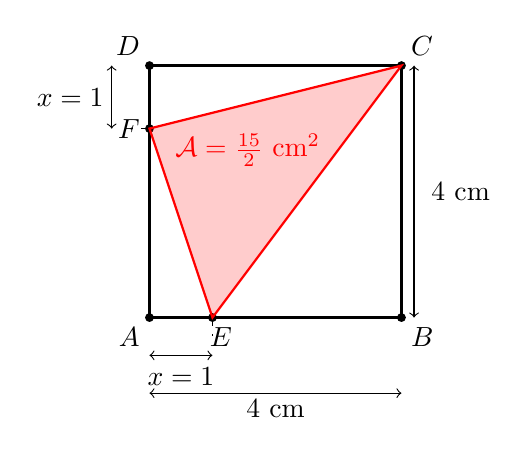
\begin{tikzpicture}[scale=0.8]
% Carré ABCD
\draw[thick] (0,0) rectangle (4,4);

% Points du carré
\fill (0,0) circle (2pt) node[below left] {$A$};
\fill (4,0) circle (2pt) node[below right] {$B$};
\fill (4,4) circle (2pt) node[above right] {$C$};
\fill (0,4) circle (2pt) node[above left] {$D$};

% Point E sur AB avec x=1
\fill (1,0) circle (2pt) node[below,xshift=3pt] {$E$};
\draw[dashed] (1,0) -- (1,-0.3);
\draw[<->] (0,-0.6) -- (1,-0.6);
\node[yshift=-10pt] at (0.5,-0.5) {$x=1$};

% Point F sur AD avec DF=x=1
\fill (0,3) circle (2pt) node[left] {$F$};
\draw[dashed] (0,3) -- (-0.3,3);
\draw[<->] (-0.6,3) -- (-0.6,4);
\node[xshift=-15pt] at (-0.6,3.5) {$x=1$};

% Triangle FEC
\draw[red,thick] (0,3) -- (1,0) -- (4,4) -- cycle;
\fill[red,opacity=0.2] (0,3) -- (1,0) -- (4,4) -- cycle;

% Dimensions du carré
\draw[<->] (4.2,0) -- (4.2,4);
\node[xshift=10pt] at (4.5,2) {$4$ cm};
\draw[<->] (0,-1.2) -- (4,-1.2);
\node[yshift=-10pt] at (2,-1) {$4$ cm};

\node[red,yshift=15pt,xshift=-10pt] at (2,2) {$\mathcal{A}=\frac{15}{2}$ cm$^2$};
\end{tikzpicture}

\tcbitem[title=Configuration avec aire minimale,halign=center]
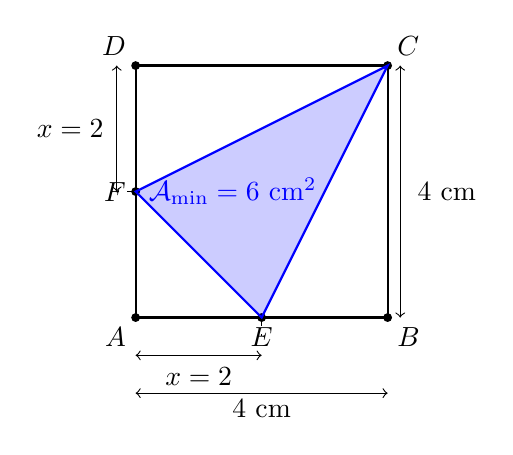
\begin{tikzpicture}[scale=0.8]
% Carré ABCD
\draw[thick] (0,0) rectangle (4,4);

% Points du carré
\fill (0,0) circle (2pt) node[below left] {$A$};
\fill (4,0) circle (2pt) node[below right] {$B$};
\fill (4,4) circle (2pt) node[above right] {$C$};
\fill (0,4) circle (2pt) node[above left] {$D$};

% Point E sur AB avec x=2
\fill (2,0) circle (2pt) node[below] {$E$};
\draw[dashed] (2,0) -- (2,-0.3);
\draw[<->] (0,-0.6) -- (2,-0.6);
\node[yshift=-10pt] at (1,-0.5) {$x=2$};

% Point F sur AD avec DF=x=2
\fill (0,2) circle (2pt) node[left] {$F$};
\draw[dashed] (0,2) -- (-0.3,2);
\draw[<->] (-0.3,2) -- (-0.3,4);
\node[xshift=-10pt] at (-0.6,3) {$x=2$};

% Triangle FEC optimal
\draw[blue,thick] (0,2) -- (2,0) -- (4,4) -- cycle;
\fill[blue,opacity=0.2] (0,2) -- (2,0) -- (4,4) -- cycle;

% Dimensions du carré
\draw[<->] (4.2,0) -- (4.2,4);
\node[xshift=10pt] at (4.5,2) {$4$ cm};
\draw[<->] (0,-1.2) -- (4,-1.2);
\node[yshift=-10pt] at (2,-1) {$4$ cm};

\node[blue,xshift=-15pt] at (2.2,2) {$\mathcal{A}_{\min}=6$ cm$^2$};
\end{tikzpicture}
\end{MultiColonnes}
\begin{tcbenumerate}[2]
\tcbitem[raster multicolumn=2] \textbf{Calcul de l'aire du triangle $FEC$ :} 

\begin{MultiColonnes}{2}
\tcbitem $\text{Aire}_{FEC} = \text{Aire du carré} - \text{Aire des autres triangles}$

L'aire du carré $ABCD$ est : $4 \times 4 = 16$ cm$^2$ ; de plus : 

\begin{MultiColonnes}{1}
    \tcbitem $\text{Aire}_{AFE} = \dfrac{1}{2} \times x \times (4-x) = \dfrac{1}{2}x(4-x) =  {\color{blue}\dfrac{1}{2}(4x-x^2)}$

    \tcbitem $\text{Aire}_{EBC} = \dfrac{1}{2} \times (4-x) \times 4 = 2(4-x) =  {\color{red}8-2x}$

    \tcbitem $\text{Aire}_{FDC} = \dfrac{1}{2} \times x \times 4 =  {\color{defi}2x}$

\end{MultiColonnes}

\tcbitem Donc :
$\text{Aire}_{FEC} = 16 - \text{Aire}_{AFE} - \text{Aire}_{EBC} - \text{Aire}_{FDC}$

$= 16 -  {\color{blue}\dfrac{1}{2}(4x-x^2)} - ( {\color{red}8-2x}) -  {\color{defi}2x}$

$= 16 - 2x + \dfrac{x^2}{2} - 8 + 2x - 2x$

$= 16 - 8 + \dfrac{x^2}{2} - 2x$

$= 8 + \dfrac{x^2}{2} - 2x = \dfrac{1}{2}(x^2 - 4x + 16)$
\end{MultiColonnes}



\tcbitem \textbf{Forme canonique et minimum :} 

$A_{FEC}(x) = \dfrac{1}{2}(x^2 - 4x + 16)$

Mettons sous forme canonique :
$x^2 - 4x + 16 = (x-2)^2 - 4 + 16 = (x-2)^2 + 12$

Donc : $A_{FEC}(x) = \dfrac{1}{2}((x-2)^2 + 12) = \dfrac{1}{2}(x-2)^2 + 6$


\tcbitem \textbf{Conclusion :} 

Le minimum de $A_{FEC}(x)$ est atteint quand $(x-2)^2 = 0$, c'est-à-dire pour $x = 2$.

La valeur minimale de l'aire est $A_{FEC}(2) = 6$ cm$^2$.

\textbf{Réponse :} L'aire du triangle $FEC$ est minimale pour $x = 2$ cm.
\end{tcbenumerate}
\end{EXO}

\newpage
\newcommand{\aideExoTrois}{
    \begin{bfbox}{Aide de l'exercice 3 :}
        \begin{tcbenumerate}[2]
            \tcbitem Faire une figure représentant la situation.
            \tcbitem Justifier l'égalité : $A_{EBC}(x)=8-2x$
            \tcbitem Montrer que l'aire du triangle $FEC$ vaut : $$A_{FEC}(x)=\dfrac{1}{2}\left(x^2-4x+16\right)$$
            \tcbitem En déduire la forme canonique de $A_{FEC}$
            \tcbitem[raster multicolumn=2] Déterminer la valeur de $x$ pour que l'aire du triangle $FEC$ soit minimale.
        \end{tcbenumerate}
    \end{bfbox}
}

\aideExoTrois
\vfill
\aideExoTrois
\vfill
\aideExoTrois
\vfill
\aideExoTrois
\vfill
\aideExoTrois
\vfill
\phantom{a}
% : \begin{EXO}{Différentes formes des polynômes de degré 2}{}%8 points 
Soit $f$ la fonction définie sur $\R$ par $ f(x) = 2x^2+4x-16$.

\begin{tcbenumerate}
\tcbitem \tcbitempoint{2}Montrer que pour tout réel $x$, $f(x) = (2x-4)(x+4)$.
\tcbitem \tcbitempoint{2}Montrer que pour tout réel $x$, $f(x) = 2(x+1)^2-18$.
\tcbitem[boxrule=0.4pt,colframe=black] Choisir la forme la plus adaptée pour répondre aux questions suivantes, puis y répondre.
\begin{tcbenumerate}[2][1][alph]
\tcbitem \tcbitempoint{1}Dresser le tableau de variations de $f$
\tcbitem \tcbitempoint{1}Résoudre $f(x)=-16$
\tcbitem \tcbitempoint{1}Dresser le tableau de signes de $f$
\tcbitem \tcbitempoint{1}Résoudre $f(x)>0$
\end{tcbenumerate}
\end{tcbenumerate}

\exocorrection

\begin{tcbenumerate}[2]
\tcbitem Montrer que pour tout réel $x$, $f(x) = (2x-4)(x+4)$.
Développons $(2x-4)(x+4)$ :
\begin{align*}
(2x-4)(x+4) &= 2x \times x + 2x \times 4 - 4 \times x - 4 \times 4\\
&= 2x^2 + 8x - 4x - 16\\
&= 2x^2 + 4x - 16\\
&= f(x)
\end{align*}

\tcbitem Montrer que pour tout réel $x$, $f(x) = 2(x+1)^2-18$.

Développons $2(x+1)^2-18$ :
\begin{align*}
2(x+1)^2-18 &= 2(x^2 + 2x + 1) - 18\\
&= 2x^2 + 4x + 2 - 18\\
&= 2x^2 + 4x - 16\\
&= f(x)
\end{align*}

\tcbitem[raster multicolumn=2] Choisir la forme la plus adaptée pour répondre aux questions suivantes :

\begin{tcbenumerate}[3][1][alph]
\tcbitem[raster multicolumn=3] Dresser le tableau de variations de $f$

\begin{MultiColonnes}{3}
    \tcbitem \textbf{Forme canonique :} 
    
Le sommet est en $(-1; -18)$ et $a = 2 > 0$, donc la parabole est tournée vers le haut.
    \tcbitem[halign=center,valign=center,raster multicolumn=2] \begin{tikzpicture}
\tkzTabInit{$x$/1,$f$/1.8}
{$-\infty$,$-1$,$+\infty$}
\tkzTabVar{+/$+\infty$,-/$-18$,+/$+\infty$}
\end{tikzpicture}
\end{MultiColonnes}

\tcbitem[raster multicolumn=1] Résoudre $f(x)=-16$

\textbf{Forme développée :} 

$2x^2+4x-16 = -16$

$2x^2+4x = 0$

$2x(x+2) = 0$

Donc $x = 0$ ou $x = -2$.

$S = \{-2 ; 0\}$

\begin{tcbenumerate}[1][4][alph]
    \tcbitem[raster multicolumn=3] Résoudre $f(x)>0$

D'après le tableau de signes précédent :

$S = \CrochetD-\infty;-4\,\,\CrochetG \cup \CrochetD2;+\infty\,\,\CrochetG$

\end{tcbenumerate}

\tcbitem[raster multicolumn=2] Dresser le tableau de signes de $f$

\textbf{Forme factorisée :} $f(x) = (2x-4)(x+4) = 2(x-2)(x+4)$ \\

Les racines sont $x = 2$ et $x = -4$.\\

\begin{tikzpicture}
\tkzTabInit{$x$/1,$2$/1,$(x+4)$/1,$(x-2)$/1,$f(x)$/1}
{$-\infty$,$-4$,$2$,$+\infty$}
\tkzTabLine{,+,t,+,t,+,}
\tkzTabLine{,-,z,+,t,+,}
\tkzTabLine{,-,t,-,z,+,}
\tkzTabLine{,+,z,-,z,+,}
\end{tikzpicture}
\end{tcbenumerate}
\end{tcbenumerate}

\end{EXO}
\begin{EXO}{Lecture graphique}{}%6 points 

\begin{MultiColonnes}{3}
\tcbitem[raster multicolumn=2] Soit $f$ la fonction dont la représentation graphique est donnée ci-contre. 

\begin{tcbenumerate}
\tcbitem \tcbitempoint{1}Lire les coordonnées du sommet $S$ de la parabole.
\tcbitem \tcbitempoint{2}Déterminer la forme canonique de $f$.
\tcbitem \tcbitempoint{1}Déterminer les racines de la fonction $f$.
\tcbitem \tcbitempoint{2}En déduire la forme factorisée de la fonction $f$.
\end{tcbenumerate}

\tcbitem[halign=center,valign=center] \begin{tikzpicture}[line cap=round,line join=round,>=triangle 45,x=1.5cm,y=1.0cm,scale=0.8]
\begin{axis}[
x=1.5cm,y=1.0cm,
axis lines=middle,
ymajorgrids=true,
xmajorgrids=true,
xmin=-1.5,
xmax=3.5,
ymin=-2.5,
ymax=3.5,
xtick={-1.0,0.0,...,3.0},
ytick={-2.0,-1.0,...,3.0},]
\clip(-1.5,-2.5) rectangle (3.5,3.5);
\draw[line width=2.pt,color=blue,smooth,samples=100,domain=-1.5:3.5] plot(\x,{-2.0*((\x)-1.0)^(2.0)+2.0});
\begin{scriptsize}
\draw[color=blue] (2,2) node {$\mathcal{C}_f$};
%\draw [fill=black] (1.,2.) circle (3.0pt);
%\draw[color=black] (0.9,2.55) node {$A$};
%\draw [fill=black] (0.,0.) circle (3.0pt);
%\draw[color=black] (0.34,4.43) node {$B$};
\end{scriptsize}
\end{axis}
\end{tikzpicture}
\end{MultiColonnes}
\exocorrection

\begin{tcbenumerate}[2]
\tcbitem Coordonnées du sommet $S$ de la parabole.

En lisant le graphique, le sommet $S$ se trouve au point le plus haut de la parabole.

$S(1 ; 2)$

\tcbitem Forme canonique de $f$.

D'après la lecture graphique :
- Sommet : $S(1 ; 2)$
- La parabole est tournée vers le bas donc $a < 0$

Pour déterminer $a$, utilisons un autre point de la courbe.
La parabole passe par $(0 ; 0)$.

$f(x) = a(x-1)^2 + 2$

$f(0) = a(0-1)^2 + 2 = a + 2 = 0$

Donc $a = -2$.

$f(x) = -2(x-1)^2 + 2$

\tcbitem Racines de la fonction $f$.

Les racines correspondent aux points d'intersection avec l'axe des abscisses, c'est-à-dire quand $f(x) = 0$.

En lisant le graphique, la parabole coupe l'axe des abscisses en $x = 0$ et $x = 2$.

Les racines sont : $x_1 = 0$ et $x_2 = 2$.

\tcbitem Forme factorisée de la fonction $f$.

Connaissant les racines $x_1 = 0$ et $x_2 = 2$, la forme factorisée est :

$f(x) = a(x-x_1)(x-x_2) = a \cdot x(x-2)$

Pour déterminer $a$, utilisons le sommet $S(1 ; 2)$ :

$f(1) = a \cdot 1 \cdot (1-2) = a \cdot 1 \cdot (-1) = -a = 2$

Donc $a = -2$.

$f(x) = -2x(x-2) = -2x^2 + 4x$

\end{tcbenumerate}

\end{EXO}
\def\rdifficulty{2}
\begin{EXO}{Problème de géométrie}{}%6 points 


$ABCD$ est un carré de coté $4$cm. Soit $x\in \CrochetG 0;4\,\,\CrochetD$. 

\begin{MultiColonnes}{2}
\tcbitem $E$ est le point de $\CrochetG AB\,\,\CrochetD$ tel que $AE=x$.
\tcbitem $F$ est le point de $\CrochetG AD\,\,\CrochetD$ tel que $DF=x$.
\end{MultiColonnes}


\tcbitempoint{6}Déterminer la valeur de $x$ pour que l'aire du triangle $FEC$ soit \acc{minimale}.


\textit{Si vous bloquez sur cette exercice, une aide est disponible sur le bureau du professeur. }

\textit{Le barème de l'exercice sera adapté ( -1 point ) si vous choisissez d'utiliser cette aide.}
\exocorrection

\begin{MultiColonnes}{2}
\tcbitem[title=Configuration générale,halign=center]
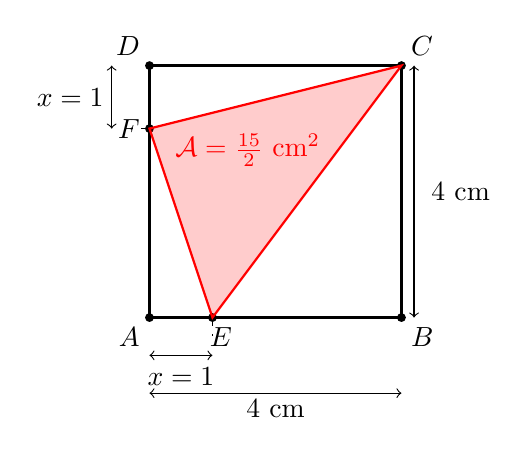
\begin{tikzpicture}[scale=0.8]
% Carré ABCD
\draw[thick] (0,0) rectangle (4,4);

% Points du carré
\fill (0,0) circle (2pt) node[below left] {$A$};
\fill (4,0) circle (2pt) node[below right] {$B$};
\fill (4,4) circle (2pt) node[above right] {$C$};
\fill (0,4) circle (2pt) node[above left] {$D$};

% Point E sur AB avec x=1
\fill (1,0) circle (2pt) node[below,xshift=3pt] {$E$};
\draw[dashed] (1,0) -- (1,-0.3);
\draw[<->] (0,-0.6) -- (1,-0.6);
\node[yshift=-10pt] at (0.5,-0.5) {$x=1$};

% Point F sur AD avec DF=x=1
\fill (0,3) circle (2pt) node[left] {$F$};
\draw[dashed] (0,3) -- (-0.3,3);
\draw[<->] (-0.6,3) -- (-0.6,4);
\node[xshift=-15pt] at (-0.6,3.5) {$x=1$};

% Triangle FEC
\draw[red,thick] (0,3) -- (1,0) -- (4,4) -- cycle;
\fill[red,opacity=0.2] (0,3) -- (1,0) -- (4,4) -- cycle;

% Dimensions du carré
\draw[<->] (4.2,0) -- (4.2,4);
\node[xshift=10pt] at (4.5,2) {$4$ cm};
\draw[<->] (0,-1.2) -- (4,-1.2);
\node[yshift=-10pt] at (2,-1) {$4$ cm};

\node[red,yshift=15pt,xshift=-10pt] at (2,2) {$\mathcal{A}=\frac{15}{2}$ cm$^2$};
\end{tikzpicture}

\tcbitem[title=Configuration avec aire minimale,halign=center]
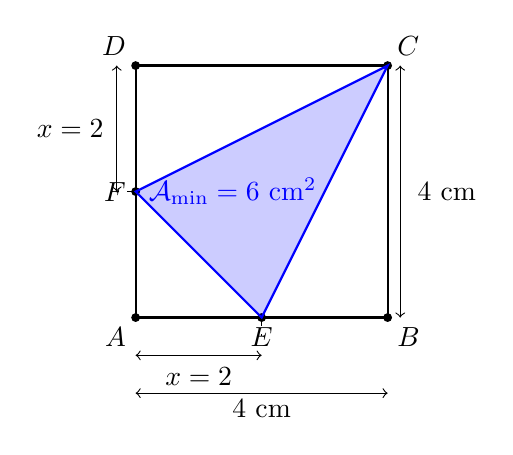
\begin{tikzpicture}[scale=0.8]
% Carré ABCD
\draw[thick] (0,0) rectangle (4,4);

% Points du carré
\fill (0,0) circle (2pt) node[below left] {$A$};
\fill (4,0) circle (2pt) node[below right] {$B$};
\fill (4,4) circle (2pt) node[above right] {$C$};
\fill (0,4) circle (2pt) node[above left] {$D$};

% Point E sur AB avec x=2
\fill (2,0) circle (2pt) node[below] {$E$};
\draw[dashed] (2,0) -- (2,-0.3);
\draw[<->] (0,-0.6) -- (2,-0.6);
\node[yshift=-10pt] at (1,-0.5) {$x=2$};

% Point F sur AD avec DF=x=2
\fill (0,2) circle (2pt) node[left] {$F$};
\draw[dashed] (0,2) -- (-0.3,2);
\draw[<->] (-0.3,2) -- (-0.3,4);
\node[xshift=-10pt] at (-0.6,3) {$x=2$};

% Triangle FEC optimal
\draw[blue,thick] (0,2) -- (2,0) -- (4,4) -- cycle;
\fill[blue,opacity=0.2] (0,2) -- (2,0) -- (4,4) -- cycle;

% Dimensions du carré
\draw[<->] (4.2,0) -- (4.2,4);
\node[xshift=10pt] at (4.5,2) {$4$ cm};
\draw[<->] (0,-1.2) -- (4,-1.2);
\node[yshift=-10pt] at (2,-1) {$4$ cm};

\node[blue,xshift=-15pt] at (2.2,2) {$\mathcal{A}_{\min}=6$ cm$^2$};
\end{tikzpicture}
\end{MultiColonnes}
\begin{tcbenumerate}[2]
\tcbitem[raster multicolumn=2] \textbf{Calcul de l'aire du triangle $FEC$ :} 

\begin{MultiColonnes}{2}
\tcbitem $\text{Aire}_{FEC} = \text{Aire du carré} - \text{Aire des autres triangles}$

L'aire du carré $ABCD$ est : $4 \times 4 = 16$ cm$^2$ ; de plus : 

\begin{MultiColonnes}{1}
    \tcbitem $\text{Aire}_{AFE} = \dfrac{1}{2} \times x \times (4-x) = \dfrac{1}{2}x(4-x) =  {\color{blue}\dfrac{1}{2}(4x-x^2)}$

    \tcbitem $\text{Aire}_{EBC} = \dfrac{1}{2} \times (4-x) \times 4 = 2(4-x) =  {\color{red}8-2x}$

    \tcbitem $\text{Aire}_{FDC} = \dfrac{1}{2} \times x \times 4 =  {\color{defi}2x}$

\end{MultiColonnes}

\tcbitem Donc :
$\text{Aire}_{FEC} = 16 - \text{Aire}_{AFE} - \text{Aire}_{EBC} - \text{Aire}_{FDC}$

$= 16 -  {\color{blue}\dfrac{1}{2}(4x-x^2)} - ( {\color{red}8-2x}) -  {\color{defi}2x}$

$= 16 - 2x + \dfrac{x^2}{2} - 8 + 2x - 2x$

$= 16 - 8 + \dfrac{x^2}{2} - 2x$

$= 8 + \dfrac{x^2}{2} - 2x = \dfrac{1}{2}(x^2 - 4x + 16)$
\end{MultiColonnes}



\tcbitem \textbf{Forme canonique et minimum :} 

$A_{FEC}(x) = \dfrac{1}{2}(x^2 - 4x + 16)$

Mettons sous forme canonique :
$x^2 - 4x + 16 = (x-2)^2 - 4 + 16 = (x-2)^2 + 12$

Donc : $A_{FEC}(x) = \dfrac{1}{2}((x-2)^2 + 12) = \dfrac{1}{2}(x-2)^2 + 6$


\tcbitem \textbf{Conclusion :} 

Le minimum de $A_{FEC}(x)$ est atteint quand $(x-2)^2 = 0$, c'est-à-dire pour $x = 2$.

La valeur minimale de l'aire est $A_{FEC}(2) = 6$ cm$^2$.

\textbf{Réponse :} L'aire du triangle $FEC$ est minimale pour $x = 2$ cm.
\end{tcbenumerate}
\end{EXO}

\newpage
\newcommand{\aideExoTrois}{
    \begin{bfbox}{Aide de l'exercice 3 :}
        \begin{tcbenumerate}[2]
            \tcbitem Faire une figure représentant la situation.
            \tcbitem Justifier l'égalité : $A_{EBC}(x)=8-2x$
            \tcbitem Montrer que l'aire du triangle $FEC$ vaut : $$A_{FEC}(x)=\dfrac{1}{2}\left(x^2-4x+16\right)$$
            \tcbitem En déduire la forme canonique de $A_{FEC}$
            \tcbitem[raster multicolumn=2] Déterminer la valeur de $x$ pour que l'aire du triangle $FEC$ soit minimale.
        \end{tcbenumerate}
    \end{bfbox}
}

\aideExoTrois
\vfill
\aideExoTrois
\vfill
\aideExoTrois
\vfill
\aideExoTrois
\vfill
\aideExoTrois
\vfill
\phantom{a}
,


\end{document}